% Task 5: two requests with the same MD5. Values from Task5/ (python3 hashlib, 2026-11-15).
% CHECKED: request_a.bin and request_b.bin are 308 bytes, differ in bytes 19, 45, 59, 83, 109, 123
%   (87/07, 71/f1, f2/72, b4/34, a8/28, 2b/ab); MD5 of both 7e58325ffced260e7cf07eb336bf0907;
%   SHA-256 99cfc680... and 748ac700...; the first 128 bytes are the MD5 collision of Wang et al. (2004)
\documentclass[12pt,tikz,border=6pt]{standalone}
% Shared preamble of the task figures of Lecture 12.
% The colours and styles are copied from the preamble of ../main.tex (keep them in sync).
% Colour mapping of Lecture 12:
%   S1 indigo: Alice (signs code and mail; in HTTPS the client)   S2 pink: Mallory, a fake certificate
%   S3 violet: a certificate                  S4 amber: a private key (black text)
%   S5 teal: Bob (checks code and mail; in HTTPS owns the website)   S6 brown: a CA or a TSA
\usepackage{lmodern}
\usepackage[T1]{fontenc}
\renewcommand{\familydefault}{\sfdefault}
\usepackage{amsmath,amssymb}
\usepackage{xcolor}
\usepackage{fontawesome5}
\usetikzlibrary{arrows.meta, calc, positioning, fit, decorations.pathreplacing, backgrounds, shadows}

\definecolor{DeepBlue}{HTML}{283593}
\definecolor{AccentOrange}{HTML}{EB5A14}
\definecolor{LightGray}{HTML}{F5F6FA}
\definecolor{sIndigo}{HTML}{5C6BC0}
\definecolor{sPink}{HTML}{EC407A}
\definecolor{sViolet}{HTML}{7E57C2}
\definecolor{sAmber}{HTML}{FFB300}
\definecolor{sTeal}{HTML}{26A69A}
\definecolor{sBrown}{HTML}{8D6E63}
\definecolor{sPinkText}{HTML}{C2185B}
\definecolor{sAmberText}{HTML}{A06A00}
\definecolor{sTealText}{HTML}{00796B}
\definecolor{aExec}{HTML}{43A047}
\definecolor{aRead}{HTML}{1E88E5}
\definecolor{aWrite}{HTML}{E53935}
\definecolor{nInk}{HTML}{37474F}
\definecolor{nLine}{HTML}{90A4AE}
\definecolor{nLight}{HTML}{CFD8DC}
\definecolor{nFill}{HTML}{ECEFF1}
\definecolor{nIdle}{HTML}{E0E0E0}

\tikzset{
  hw/.style={draw=nLine, thick, fill=nFill, text=nInk, rounded corners=3pt, align=center, inner sep=4pt},
  hwmain/.style={draw=nInk, thick, fill=nInk, text=white, rounded corners=3pt, align=center, inner sep=4pt},
  container/.style={draw=nLine, thick, dashed, rounded corners=5pt},
  actor/.style={fill=#1, draw=#1, text=white, rounded corners=3pt, align=center, font=\small\bfseries, inner sep=5pt},
  actorlight/.style={fill=#1!15, draw=#1, thick, text=nInk, rounded corners=3pt, align=center, inner sep=5pt},
  person/.style={circle, fill=#1, draw=#1, text=white, minimum size=1.1cm, font=\Large, inner sep=0pt},
  data/.style={-{Stealth}, very thick, nInk},
  flow/.style={-{Stealth}, very thick, DeepBlue},
  annot/.style={draw=AccentOrange, line width=1.6pt, rounded corners=3pt},
  note/.style={font=\small, text=nInk},
  % a certificate card: violet frame, light violet fill
  cert/.style={draw=sViolet, thick, fill=sViolet!10, text=nInk, rounded corners=3pt, align=left, inner sep=5pt,
    font=\small},
  fakecert/.style={draw=sPink, thick, fill=sPink!10, text=nInk, rounded corners=3pt, align=left, inner sep=5pt,
    font=\small},
  keybox/.style={draw=sAmber, thick, fill=sAmber!25, text=black, rounded corners=3pt, align=center, inner sep=4pt},
  cabox/.style={fill=sBrown, draw=sBrown, text=white, rounded corners=3pt, align=center, font=\small\bfseries, inner sep=5pt},
  byte/.style={draw=nLine, thick, fill=white, text=nInk, font=\ttfamily\small,
    minimum width=0.72cm, minimum height=0.58cm, inner sep=1pt, rounded corners=1.5pt},
  chg/.style={byte, fill=AccentOrange!18, draw=AccentOrange, line width=1.4pt, font=\ttfamily\small\bfseries},
  rowlabel/.style={font=\small\bfseries, text=nInk, anchor=east},
}
\newcommand{\ok}{\textcolor{aExec}{\faCheck}}
\newcommand{\nok}{\textcolor{aWrite}{\faTimes}}
\newcommand{\qm}{\textcolor{AccentOrange}{\textbf{?}}}
% a file icon with a name under it: \fileicon{node name}{position}{label}
\newcommand{\fileicon}[3]{%
  \node[text=nInk, font=\fontsize{26}{28}\selectfont] (#1) at (#2) {\faFile*[regular]};
  \node[font=\scriptsize\ttfamily, text=nInk, below=0.02cm of #1] {#3};}

\begin{document}
\pagecolor{white}
\begin{tikzpicture}[>=Stealth]
  % ---------- the two requests ----------
  \foreach \x/\nm/\col/\txt/\bytes in {
      0/a/sIndigo/{shop.alice.example is a website.\\It may NOT sign certificates.}/{87,71,f2,b4,a8,2b},
      9.4/b/sPink/{Mallory is a CA. She may sign\\certificates for any website.}/{07,f1,72,34,28,ab}} {
    \node[draw=nLine, thick, fill=white, minimum width=7.6cm, minimum height=4.4cm, rounded corners=2pt] (p) at (\x,0) {};
    \node[font=\small\bfseries, text=nInk, anchor=north west] at ([shift={(0.15,-0.1)}]p.north west)
      {\faFile*[regular]\ \texttt{request\_\nm.bin}\quad\normalfont\scriptsize 308 bytes};
    \node[font=\scriptsize, text=gray, anchor=north west] at ([shift={(0.15,-0.62)}]p.north west)
      {bytes 0 to 127: strange bytes, the 6 that differ:};
    \foreach \v [count=\j from 0] in \bytes {
      \ifnum\j=0 \node[chg] at ({\x-3.05+0.9*\j},0.55) {\v};\else\node[chg] at ({\x-3.05+0.9*\j},0.55) {\v};\fi
    }
    \foreach \pos [count=\j from 0] in {19,45,59,83,109,123}
      \node[font=\tiny, text=gray] at ({\x-3.05+0.9*\j},0.1) {byte \pos};
    \node[font=\scriptsize, text=gray, anchor=west] at (\x-3.65,-0.45) {then the text, the same in both; a program shows:};
    \node[actorlight=\col, font=\small, text width=6.8cm] at (\x,-1.4) {\txt};
  }
  % ---------- the hashes ----------
  \node[hw, font=\small\ttfamily, minimum width=7.6cm] (h1) at (0,-3.2) {MD5 = ?\qquad SHA-256 = ?};
  \node[hw, font=\small\ttfamily, minimum width=7.6cm] (h2) at (9.4,-3.2) {MD5 = ?\qquad SHA-256 = ?};
  \draw[data] (0,-2.2) -- (h1.north);
  \draw[data] (9.4,-2.2) -- (h2.north);
  
  % ---------- the signature ----------
  \node[cabox] (ca) at (0,-4.9) {\faStamp\ Trusty CA signs A\\ \normalfont\scriptsize RSA over MD5 (and over SHA-256)};
  \draw[data] (h1.south) -- (ca.north);
  \draw[data, dashed, AccentOrange] (ca.east) -- node[above, font=\small\bfseries, text=AccentOrange] {does the same signature fit B?} (9.4,-4.9) -- (h2.south);
\end{tikzpicture}
\end{document}
